\documentclass{beamer}

\usepackage{skull} % for skull symbol
\usepackage{graphicx}
\usepackage{amsmath}
%\usepackage{mathabx} % for convolution symbol
\usepackage{pgfplots} % for tikzpicture
\usepackage{color}
\usepackage{tikz}
%\usepackage{pgf}
%\usetikzlibrary{shapes,matrix}
\usetikzlibrary{matrix}

\def\layersep{1.5cm}

% for colored math symbols
\newcommand*{\mathcolor}{}
\def\mathcolor#1#{\mathcoloraux{#1}}
\newcommand*{\mathcoloraux}[3]{%
  \protect\leavevmode
  \begingroup
    \color#1{#2}#3%
  \endgroup
}

\mode<notes>{
%\usetheme{Berkeley}
\definecolor{uofsgreen}{rgb}{0.125,0.5,0.25}
\usecolortheme[named=uofsgreen]{structure}
}

\setbeamerfont{page number in head/foot}{size=\large}
\setbeamertemplate{footline}[frame number]

%\title[Short Paper Title]{Dermatologist-level classification of skin cancer with deep neural networks}
%\subtitle{A. Esteva, B. Kuprel, R.A. Novoa, J. Ko, S.M. Swetter, 
%H.M. Blau, and S. Thrun} % (optional)
\title[Short Paper Title]{CNN Basics}
\subtitle{}
%\author{Shubhra Aich}
\institute{}
\author{\texorpdfstring{Shubhra Aich\newline\url{s.aich.72@gmail.com}}{Shubhra Aich}}
\date{January 17, 2018}

\begin{document}

\begin{frame}
  \titlepage
\end{frame}

\begin{frame}
  \frametitle{Outline}
  \tableofcontents
\end{frame}

%\section{Architectural Overview}

\subsection{RGB image basics}
\begin{frame}
	\frametitle{RGB image basics}
	\begin{minipage}{0.45\textwidth}	 		
	\textcolor{red}{R}\textcolor{green}{G}\textcolor{blue}{B} image consists of 3 channels or planes, namely \textcolor{red}{Red}, \textcolor{green}{Green} and \textcolor{blue}{Blue}. \\
	We see the combined effect of these channels.
	\end{minipage}	
	\begin{minipage}{0.45\textwidth}
		\hspace{1em}	
		\begin{figure}
	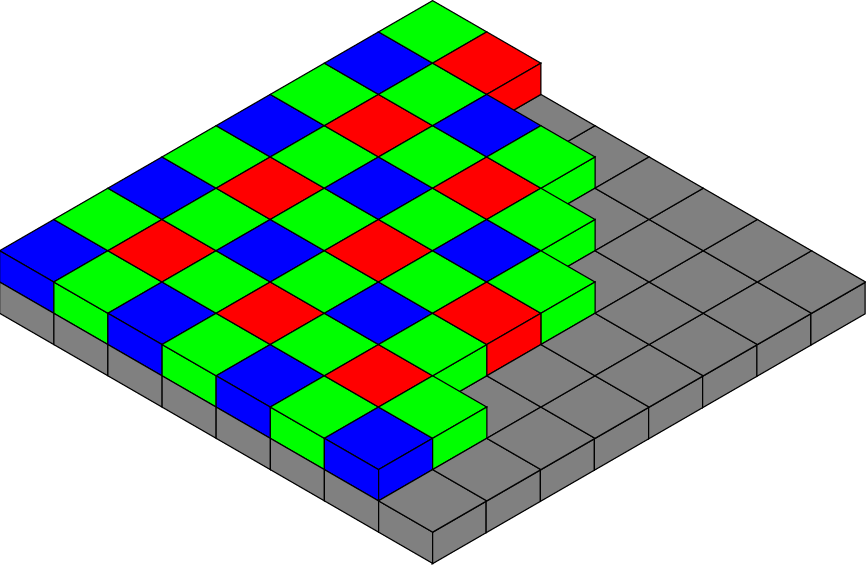
\includegraphics[scale=0.12]{./figures/edit/bayer_sensor.png} 				
	\end{figure}
			
	\end{minipage} \\
	\begin{minipage}{0.60\textwidth}	 				\begin{figure} 									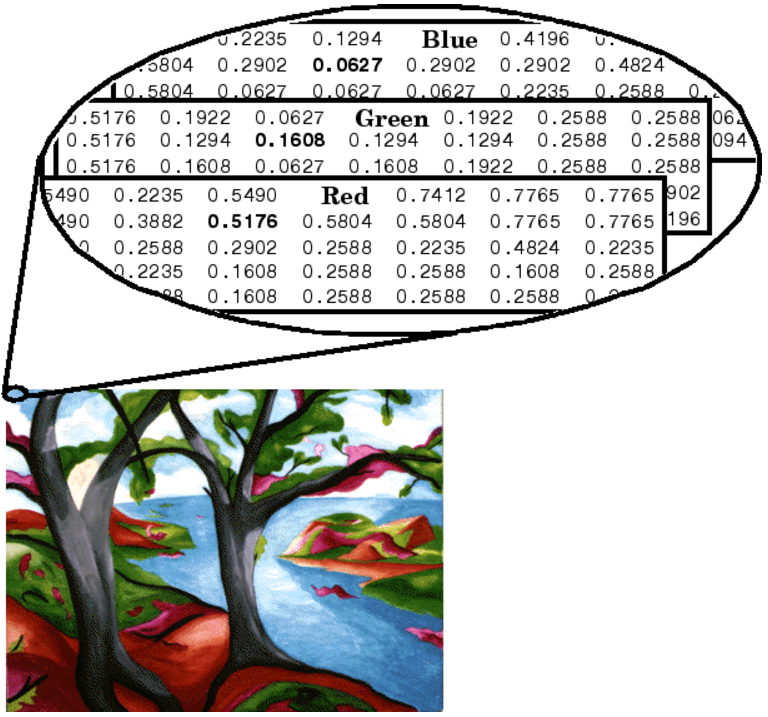
\includegraphics[width=0.7\textwidth]{./figures/edit/rgb_sample.png} 
		\end{figure}
			
	\end{minipage}
\end{frame}

\subsection{ANN vs CNN}

\begin{frame}
	\frametitle{Artifical \textit{vs} Convolutional NN}
	\begin{figure}
		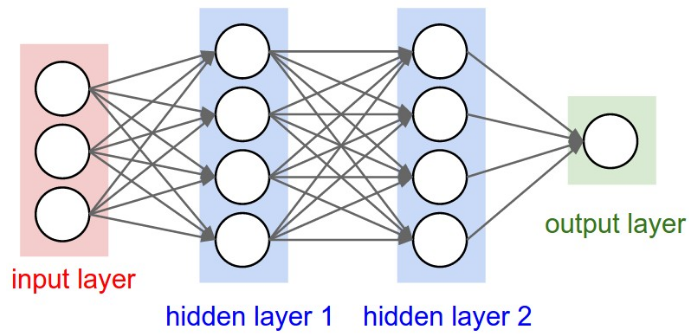
\includegraphics[scale=0.30]{./figures/edit/ann.png} \\
		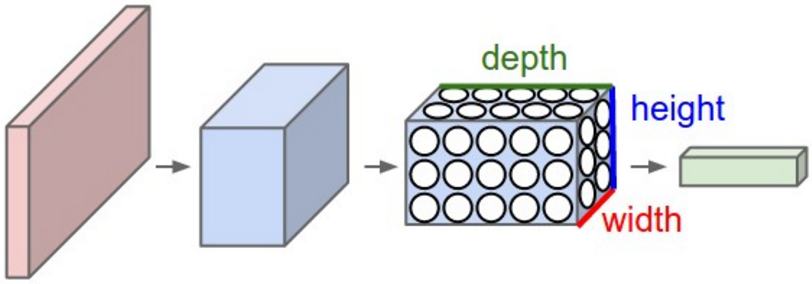
\includegraphics[scale=0.32]{./figures/edit/cnn.png} 
	\end{figure}
\end{frame}


\subsection{Operations in CNN}
\begin{frame}
	\frametitle{Operations in CNN}
	\begin{itemize}
		\item Convolution
		\item Rectification
		\item Pooling
		\item Dropout
	\end{itemize}
\end{frame}

\subsubsection{Convolution}

\begin{frame}
	\frametitle{Convolution ...(1)}
	\begin{figure}
		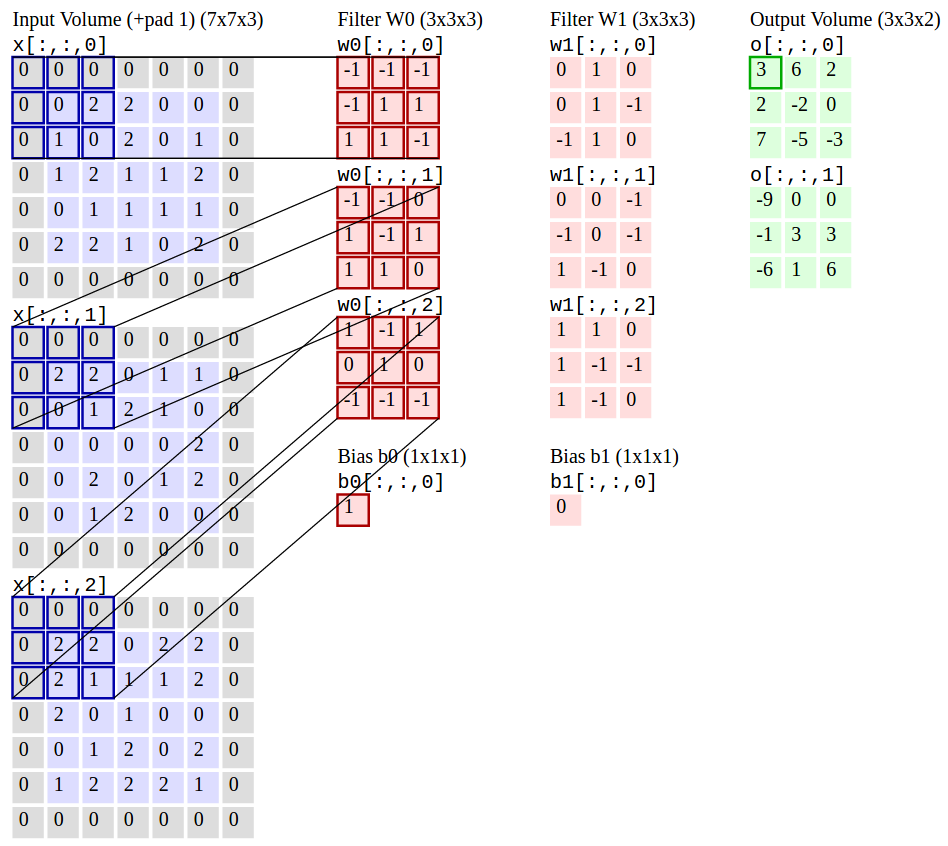
\includegraphics[scale=0.28]{./figures/edit/conv_03_edit.png}
	\end{figure}
\end{frame}

\begin{frame}
	\frametitle{Convolution ...(2)}
	\begin{figure}
		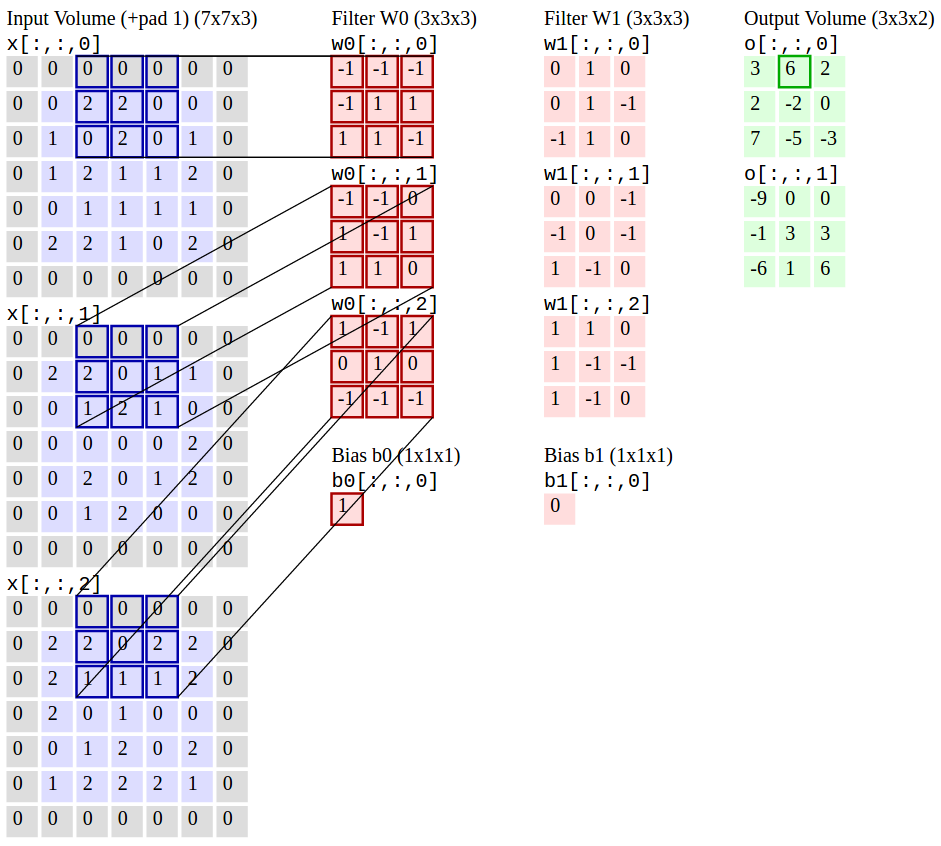
\includegraphics[scale=0.28]{./figures/edit/conv_04_edit.png}
	\end{figure}
\end{frame}

\begin{frame}
	\frametitle{Convolution ...(3)}
	\begin{figure}	
		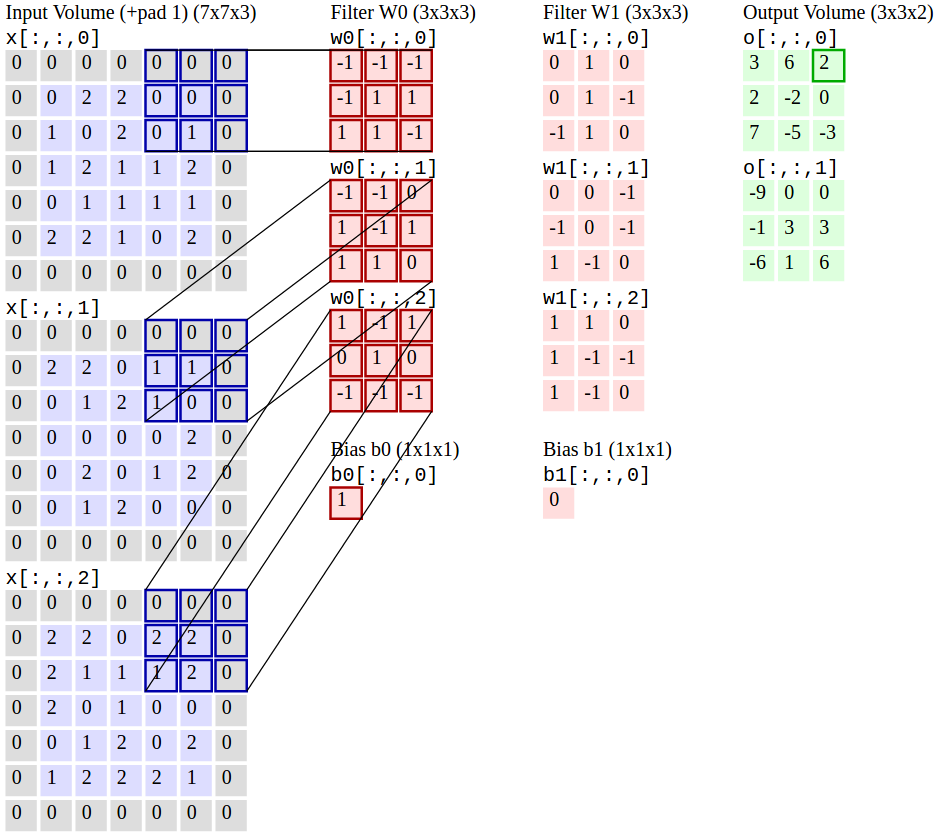
\includegraphics[scale=0.28]{./figures/edit/conv_05_edit.png}
	\end{figure}
\end{frame}

\begin{frame}
	\frametitle{Convolution ...(4)}
	\begin{figure}
		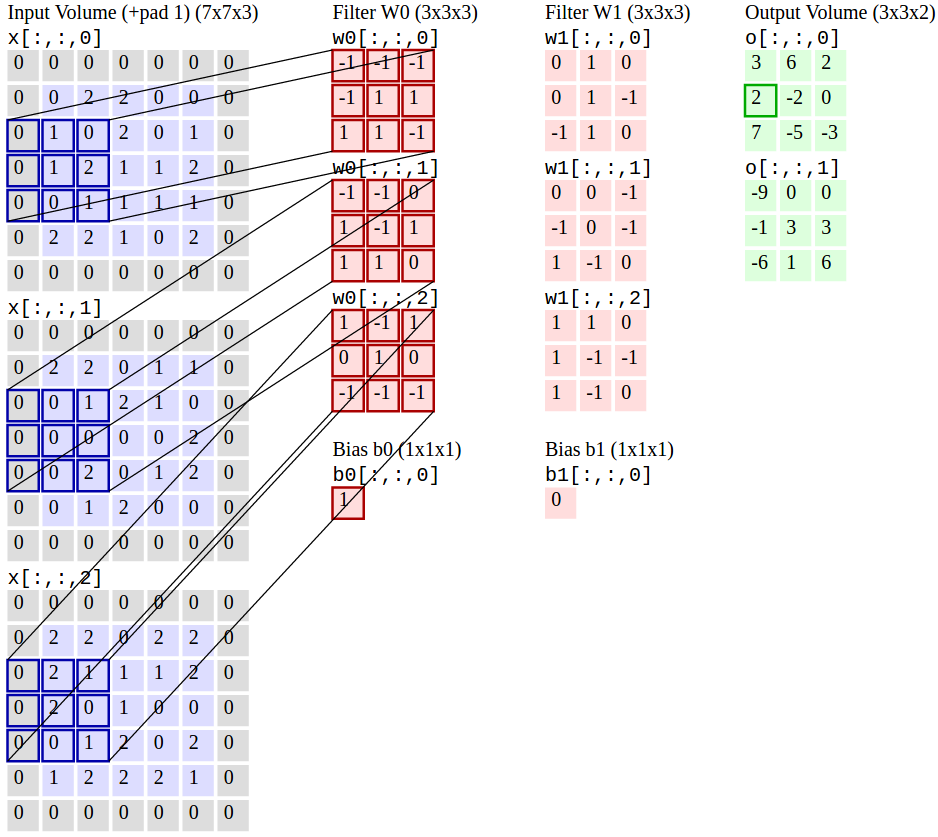
\includegraphics[scale=0.28]{./figures/edit/conv_06_edit.png}
	\end{figure}
\end{frame}

\begin{frame}
	\frametitle{Convolution ...(5)}
	\begin{figure}	
		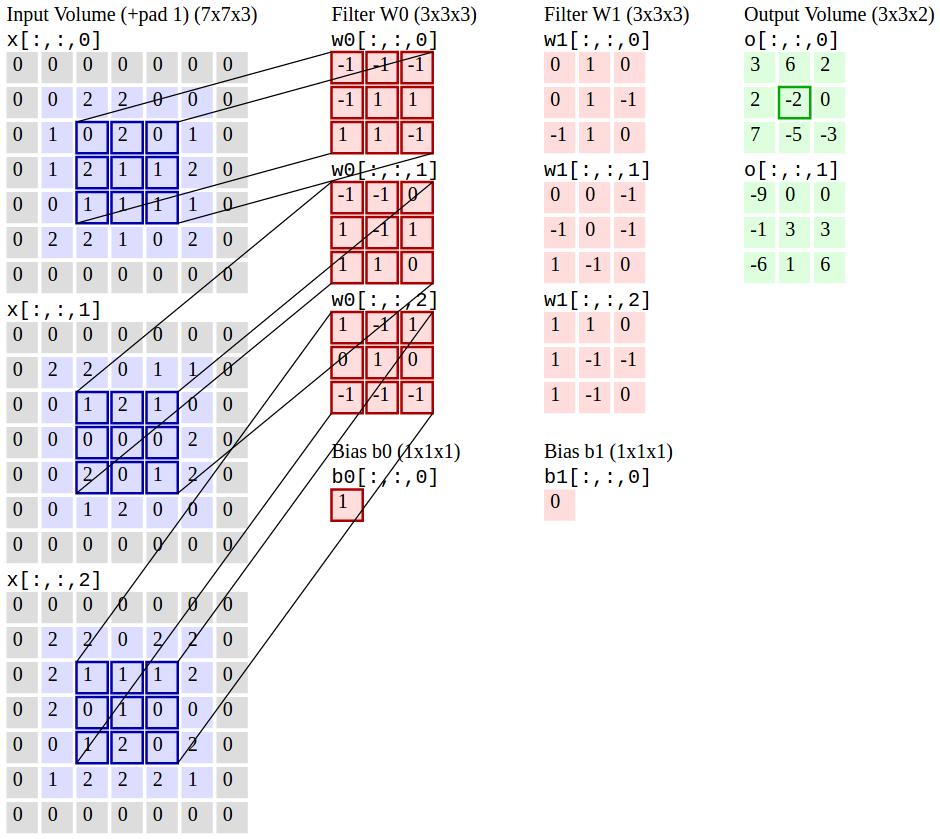
\includegraphics[scale=0.28]{./figures/edit/conv_07_edit.png}
	\end{figure}
\end{frame}

\begin{frame}
	\frametitle{Convolution ...(6)}
	\begin{figure}
		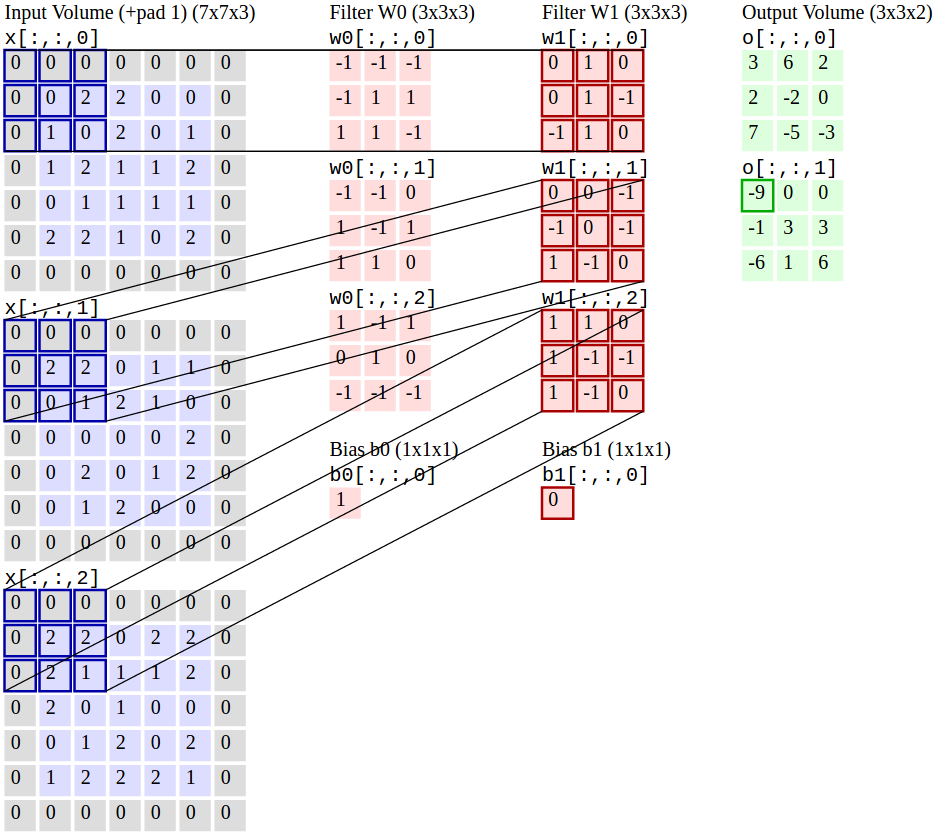
\includegraphics[scale=0.28]{./figures/edit/conv_08_edit.png}
	\end{figure}
\end{frame}

\begin{frame}
	\frametitle{Equations of Convolution}
%	\begin{figure}
%		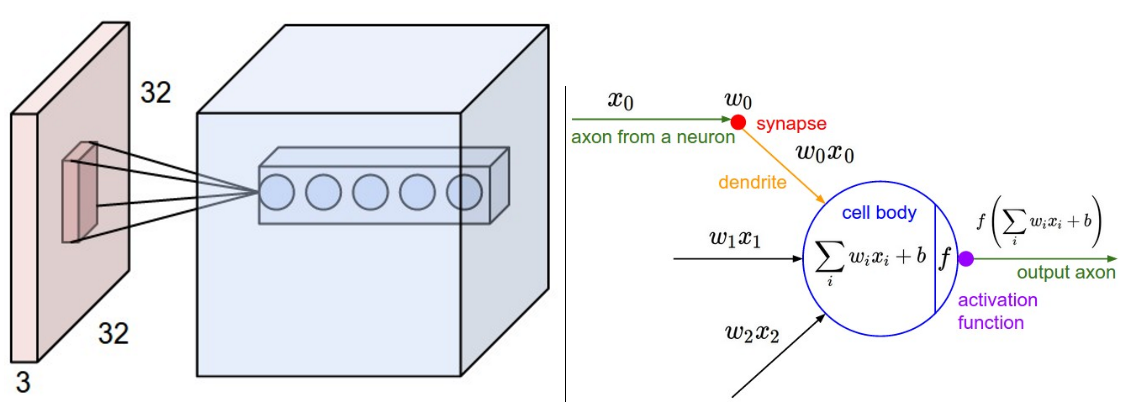
\includegraphics[scale=0.28]{./figures/edit/conv_02.png}
%	\end{figure} \\
	\begin{multiline}
		w_i = \text{weights of the filter} \\
		x_i = \text{outputs of the previous layer} \\
		z = \sum_{i} w_i x_i + b = w.x + b \mathcolor{red}{\equiv w \ast x + b} \\
		a = f(z) \\
		f = \text{activation/ rectification / squashing function} 
	\end{multiline}
\end{frame}

\subsubsection{Pooling}

\begin{frame}
	\frametitle{Pooling}
	\begin{figure}
		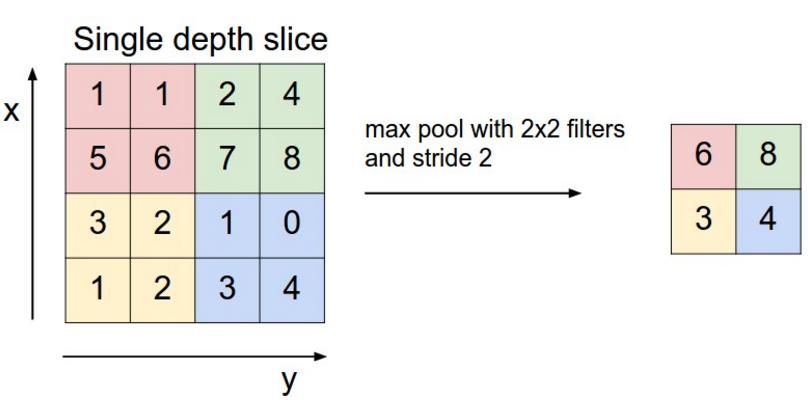
\includegraphics[scale=0.23]{./figures/edit/max_pool_short.png}
	\end{figure}	
		\begin{itemize}
		\item Max-pooling.
		\item Average pooling.
		\pause
		\item Min-pooling 
		\pause
		$\mathcolor{red}{ \skull } $
	\end{itemize}	
\end{frame}

\begin{frame}
	\frametitle{Why do we use Convolution and Pooling? ...(1)}
	CNN combines 3 architectural ideas to deal with shift, scale and distortion.
	\begin{itemize}
		\item Local receptive fields/filters 
		\begin{itemize}
			\item The idea of local filters dates back to Hubel-Wiesel's discovery of locally sensitive, orientation selective neurons in the cat's visual cortex.
			\item It helps to extract elementary visual features, such as edges, corners, end-points etc. 
		\end{itemize}
		\item Shared weights
		\begin{itemize}
			\item Distortions or shifts of the input causes the position of salient features to vary.			
			\item Elementary feature detectors that are useful on one region of the image are likely to be useful across the entire image. 
			\item This knowledge can be applied by forcing a set of units, whose receptive fields are located at different places on the to be identical.
			\item These features are combined by subsequent layers to detect more meaningful features.			
		\end{itemize}
	\end{itemize}
\end{frame}

\begin{frame}
	\frametitle{Why do we use Convolution and Pooling? ...(2)}
	\begin{itemize}
		\item Sub-sampling/Pooling
		\begin{itemize}
			\item Once a feature is detected, its exact location becomes less important, only approximate position relative to other features is relevant.
			\item This precise position is even harmful they vary from image to image.
			\item The simplest way to reduce this precision is sub-sampling or pooling.
		\end{itemize}
	\end{itemize}		  
\end{frame}

\subsubsection{Rectification}

\begin{frame}
	\frametitle{Rectification}
	\begin{itemize}
		\item Linear neuron, $ y = wx + b $
		\item Rectified linear neuron (ReLU), 
			$ y = 
			\begin{cases} 
				wx + b, & \text{if} x > 0 \\
				0, & \text{otherwise} 
			\end{cases} $
		\item Sigmoid/logistic neuron, $ y = \frac{1}{1+exp(-\alpha(wx + b))} $
		
	\end{itemize}
\begin{center}
\resizebox{8cm}{5cm}{%
\begin{tikzpicture}
    \begin{axis}%
    [
        grid=major,     
        xmin=-1,
        xmax=1,
        axis x line=bottom,
        ytick={0,.5,1},
        ymax=1,
        axis y line=middle,
    ]
        \addplot%
        [
            blue,%
            mark=none,
            samples=1000,
            domain=-1:1,
        ]
        (x,{1/(1+exp(-5*x))});
        
        \addplot%
        [
            cyan,%
            mark=none,
            samples=100,
            domain=-6:6,
        ]
        (x,{0.8*x});
        
        \addplot%
        [
            magenta,%
            mark=none,
            samples=10,
            domain=-1:0,
        ]
        (x,{0});
        \addplot%
        [
            magenta,%
            mark=none,
            samples=10,
            domain=0:1,
        ]
        (x,{1.2*x});        
    \end{axis}
\end{tikzpicture}
}
\end{center}
\end{frame}

\begin{frame}
	\frametitle{Choice of Recitification Functions }
	\begin{itemize}
		\item Backpropagation is the most popular learning algorithm for 
		a network comprising real-valued units. 
		\item This learning algorithm adjusts the weights in each iteration 		in proportion to the derivative of the final error function w.r.t. 
		the weights.
		\item To facilitate learning, rectification functions are expected 			to have more or less smooth derivatives.
		\item Linear neurons can map only linear input-output 						relationships.
		\item Linear neurons are unbounded both below and above.
		\item Sigmoid activation works well for simple ANN. However, in 
		deeper models like CNN, tiny error-gradients of sigmoid units make 			learning horrendously slow.
	\end{itemize}		
\end{frame}

\subsubsection{Dropout}

\begin{frame}
	\frametitle{Dropout}
	\begin{figure}
		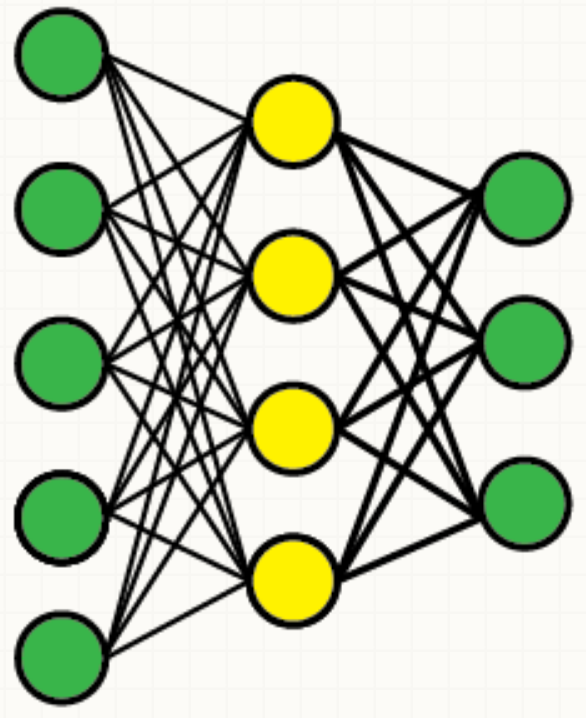
\includegraphics[width=0.25\textwidth]{./figures/edit/full_network.png}
		\hspace{1em}
		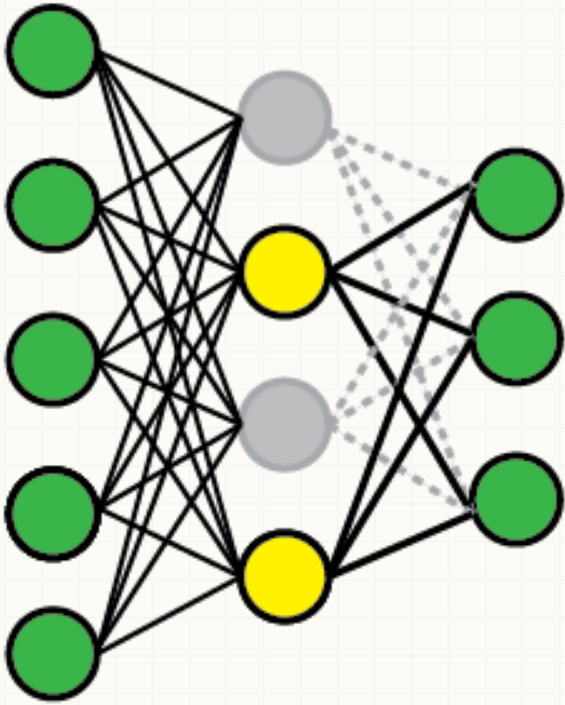
\includegraphics[width=0.25\textwidth]{./figures/edit/drop_01.png}
		\hspace{1em}		
		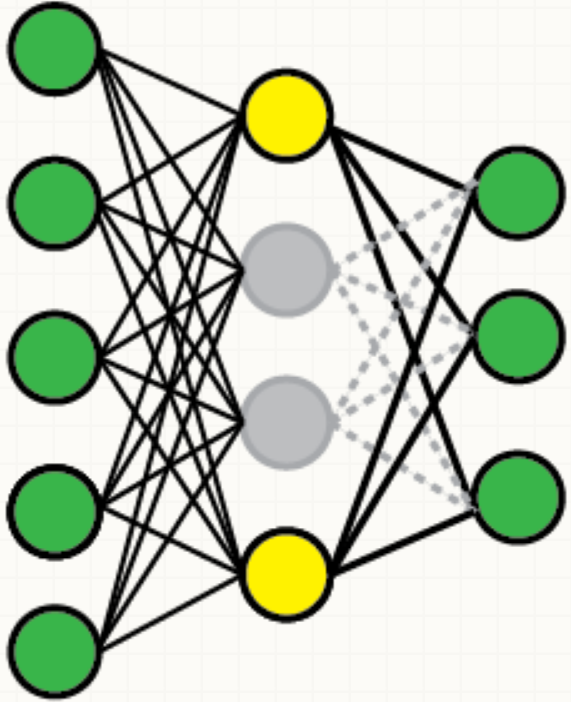
\includegraphics[width=0.25\textwidth]{./figures/edit/drop_02.png}		
	\end{figure}
	
	\begin{itemize}
		\item In each iteration of learning, we randomly omit each hidden unit with a prespecified probability.
		\item Using dropout, for a network comprising single hidden layer with H hidden units, in each iteration, we randomly sample from $2^H$ different architectures.
		\item All architectures share weights.
		\item Dropout prevents overfitting.
		\item In test time, the full network is used with parameter values halved.
	\end{itemize}
\end{frame}

\end{document}


